\section{Framing}\label{sec:framing}
When you need to send data over a network, you can't just throw it out there and hope for the best (unless you're UDP, which does exactly that). You need to package it up in a way that makes sense to the receiving device. This is where framing comes into play.

Framing is the process of encapsulating data into discrete units called frames. Each frame contains not only the actual data being sent but also additional information that helps the receiving device understand how to process it. This includes things like source and destination addresses, error-checking information, and control information. We'll go through some frame structure diagrams \textit{a lot} in this reader, so get used to it!

\section{Ethernet}
\label{sec:ethernet}
Ethernet is the most widely used local area network (LAN) technology today. It defines both the physical layer specifications (cables, connectors) and the data link layer framing protocol.

\subsection{Ethernet Frame Structure}
Remember when I said you should get used to frame structure diagrams? Well, here's one for Ethernet:

\begin{figure}[h]
    \centering
    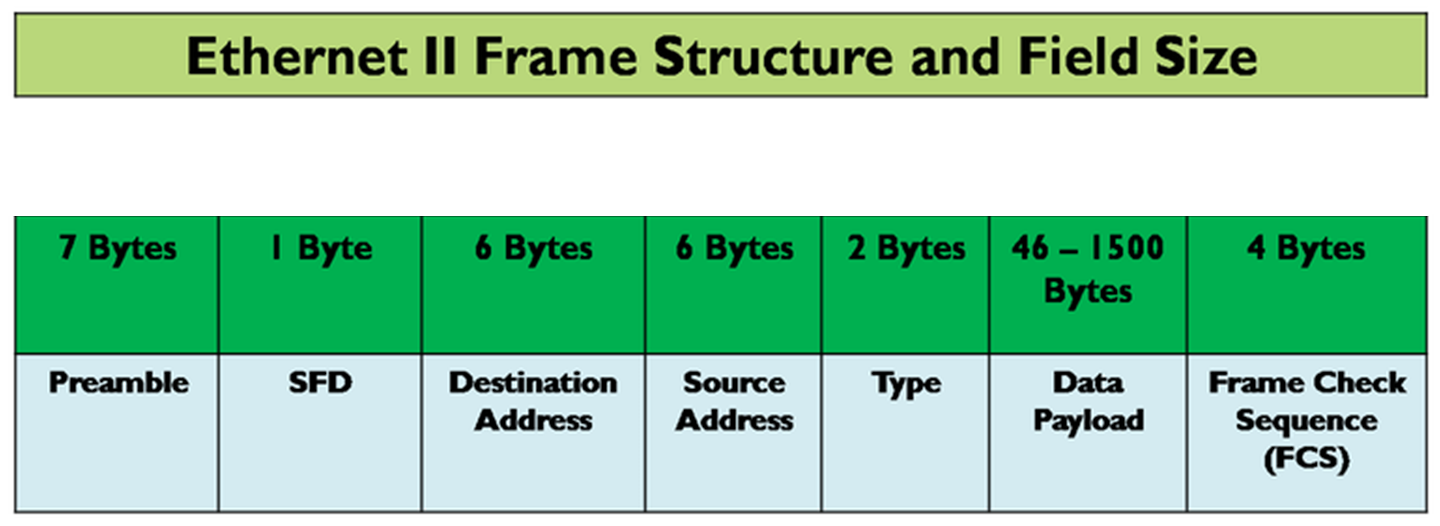
\includegraphics[width=\textwidth]{assets/osi/datalink/protocols/ethernet.png}
    \caption{Ethernet Frame Structure}
    \label{fig:ethernet_frame_structure}
\end{figure}

\begin{itemize}
\item \textbf{Preamble (7 bytes):} A sequence of alternating 1s and 0s used for synchronization
\item \textbf{Start Frame Delimiter (1 byte):} Marks the beginning of the frame with pattern 10101011
\item \textbf{Destination Address (6 bytes):} MAC address of the receiving device
\item \textbf{Source Address (6 bytes):} MAC address of the sending device
\item \textbf{Type/Length (2 bytes):} Indicates either the protocol type or frame length
\item \textbf{Data (46-1500 bytes):} The actual payload being transmitted
\item \textbf{Frame Check Sequence (4 bytes):} CRC-32 checksum for error detection
\end{itemize}


Different Ethernet standards may have variations in frame size and structure, but the basic components remain consistent. The minimum frame size is 64 bytes, and the maximum is 1518 bytes (or 1522 bytes with VLAN tagging).

\newpage
There are different physical specifications as well, which you will never need in real life, but might come across on the exam. If you need a refresher on the different types of cables, check out Section \ref{sec:transmission_media} and Table \ref{tab:ethernet_standards} below.

